\section{IP}
Utilizamos el término \textbf{internetwork}, o a veces simplemente \textbf{internet} con una i minúscula, para referirnos a una colección arbitraria de redes interconectadas para proporcionar algún tipo de servicio de entrega de paquetes de host a host.

Las internet conecta diversas redes através de routers. Es fácil confundirse con la distinción entre bridges, switches y routers. Hay una buena razón para tal confusión, ya que en algún nivel todos reenvían mensajes de un enlace a otro. Una distinción que la gente hace se basa en la estratificación: los bridges son nodos de nivel de enlace (reenvían frames de un enlace a otro para implementar una LAN extendida), los switches son nodos de nivel de red (reenvían paquetes de un enlace a otro para implementar una red conmutada por paquetes) y los routers son nodos de nivel de internet (reenvían datagramas de una red a otra para implementar un internet).

El \textbf{Protocolo de Internet (Internet Protocol - IP)} es la herramienta clave utilizada hoy en día para construir internetworks escalables y heterogéneas.
La filosofía utilizada en la definición del modelo de servicio IP fue hacerlo poco exigente para que casi cualquier tecnología de red que pueda aparecer en una internetwork pueda proporcionar el servicio necesario.

El modelo de servicio IP puede pensarse en dos partes: un esquema de direccionamiento, que proporciona una forma de identificar todos los hosts en la internetwork, y un modelo de datagrama (sin conexión) de entrega de datos. Este modelo de servicio a veces se llama mejor esfuerzo (\textbf{best effort}) porque, aunque IP hace todo lo posible para entregar datagramas, no ofrece garantías.

Cada datagrama lleva suficiente información para permitir que la red reenvíe el paquete a su destino correcto; no es necesario ningún mecanismo de configuración previa para decirle a la red qué hacer cuando llega el paquete. Simplemente lo envía y la red hace todo lo posible para llevarlo al destino deseado. La parte de "mejor esfuerzo" significa que si algo sale mal y el paquete se pierde, se corrompe, se entrega incorrectamente o de cualquier manera no llega a su destino previsto, la red no hace nada: hizo su mejor esfuerzo y eso es todo lo que tiene que hacer. No hace ningún intento de recuperarse del fallo. Esto a veces se llama un servicio no confiable.

La entrega de mejor esfuerzo no significa solo que los paquetes pueden perderse. A veces pueden entregarse fuera de orden, y a veces el mismo paquete puede entregarse más de una vez. Los protocolos de nivel superior o las aplicaciones que se ejecutan por encima de IP deben ser conscientes de todos estos posibles modos de falla.

\subsection{Formato del paquete}
Una parte clave del modelo de servicio IP es el tipo de paquetes que se pueden transportar. El datagrama IP, como la mayoría de los paquetes, consiste en una cabecera seguida de un número de bytes de datos.


\begin{figure}[H]
	\centering
	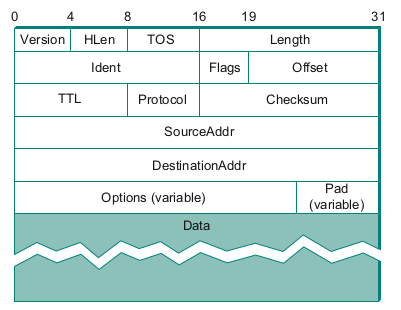
\includegraphics[width=0.5\textwidth
]{images/ip-frame.png}
	\caption[Paquete IP]{Paquete IP}
	\label{fig:ip-frame}
\end{figure}

El header del paquete consta de los siguientes campos:
\begin{itemize}
  \item El campo \textbf{Version} especifica la versión de IP. La versión actual de IP es 4, y a veces se llama IPv4. Colocar este campo justo al comienzo del datagrama facilita que todo lo demás en el formato del paquete se redefina en versiones posteriores.
  \item El campo \textbf{HLEN} especifica la longitud del encabezado en palabras de 32 bits. Cuando no hay opciones, lo que sucede en la mayoía de los casos, el encabezado tiene 5 palabras (20 bytes) de largo.
  \item El campo \textbf{TOS (tipo de servicio)} de 8 bits ha tenido una serie de definiciones diferentes a lo largo de los años, pero su función básica es permitir que los paquetes se traten de manera diferente según las necesidades de la aplicación.
  \item El campo \textbf{Length} (16 bits) contienen la longitud del datagrama, incluido el encabezado. A diferencia del campo HLen, el campo Longitud cuenta bytes en lugar de palabras. Por lo tanto, el tamaño máximo de un datagrama IP es de 65.535 bytes. Sin embargo, la red física a través de la cual se ejecuta IP puede no admitir paquetes tan largos. Por esta razón, IP admite un proceso de fragmentación y reensamblaje.
  \item Los campos \textbf{Ident}, \textbf{Flags} y \textbf{Offset} contienen información sobre la fragmentación, que se describe en la siguiente sección.
  \item El campo \textbf{TTL} es el tiempo de vida del paquete. La intención del campo es capturar paquetes que han estado dando vueltas en bucles de enrutamiento y descartarlos, en lugar de dejar que consuman recursos indefinidamente.

  Dado que no todos los enrutadores no tienen acceso a un reloj común, la mayoría de los enrutadores simplemente decrementaban el TTL en 1 a medida que envian el paquete. Por lo tanto, se convirtió más en un recuento de saltos que en un temporizador.

  Establecer este campo demasiado alto haría que los paquetes circulen bastante antes de ser descartados; Establecerlo demasiado bajo podría conllevar a que no lleguen a su destino. El valor 64 es el valor predeterminado actual.

  \item El campo \textbf{protocolo} es simplemente una clave de demultiplexión que identifica el protocolo de nivel superior al que se debe pasar este paquete IP. Hay valores definidos para el protocolo TCP (Protocolo de control de transmisión - 6), UDP (Protocolo de datagramas de usuario - 17) y muchos otros protocolos que pueden estar por encima de IP en el gráfico de protocolos.
  
  \item El campo \textbf{Checksum} es un campo de detección de errores de 16 bits que cubre tanto el encabezado como los datos. Sirve para detectar errores, no así para corregirlos. Por lo tanto, si el host detecta un error en el paquete, lo descarta.
  \item El campo \textbf{SourceAddr} es la dirección completa del host que envía el paquete. Es necesaria para permitir que los destinatarios decidan si desean aceptar el paquete y para permitirles responder.
  \item El campo \textbf{DestinationAddr} es la dirección completa del host que debe recibir el paquete.  Es la clave para la entrega de datagramas: cada paquete contiene una dirección completa para su destino previsto para que se puedan tomar decisiones de reenvío en cada enrutador.
  \item Finalmente, puede haber una serie de opciones al final del encabezado. La presencia o ausencia de opciones se puede determinar examinando el campo HLen. Si bien las opciones se usan con bastante poca frecuencia, una implementación IP completa debe poder procesarlas todas.
\end{itemize}

\subsection{Fragmentación y reensambe}
Cada tipo de red tiene una \textbf{unidad de transmisión máxima (MTU)}, que es el datagrama IP más grande que puede transportar en un frame.

Cuando un host envía un datagrama IP, por lo tanto, puede elegir cualquier tamaño que desee. Una opción razonable es el MTU de la red a la que está directamente conectado. Entonces, la fragmentación solo será necesaria si la ruta hacia el destino incluye una red con un MTU más pequeño. Si el protocolo de transporte que se encuentra en la parte superior de IP le da un paquete más grande que el MTU local, entonces el host de origen debe fragmentarlo.

Para permitir que estos fragmentos se vuelvan a ensamblar en el host de recepción, todos llevan el mismo identificador en el campo Ident. Este identificador es elegido por el host de envío y pretende ser único entre todos los datagramas que puedan llegar al destino desde esta fuente durante un período de tiempo razonable. Dado que todos los fragmentos del datagrama original contienen este identificador, el host de reensambe podrá reconocer aquellos fragmentos que van juntos. Si no llegan todos los fragmentos al host de recepción, el host abandona el proceso de reensamble y descarta los fragmentos que llegaron. IP no intenta recuperarse de fragmentos faltantes.

Supongamos que hay que fragmentar un mensaje recibido, entonces se establece el bit M en el campo Flags, lo que significa que hay más fragmentos por seguir, y establece el Offset en 0, ya que este fragmento contiene la primera parte del datagrama original.

La fragmentación produce datagramas IP más pequeños y válidos que pueden reensamblarse fácilmente en el datagrama original al recibirlos, independientemente del orden de su llegada. El reensamblaje se realiza en el host receptor y no en cada enrutador.

\subsection{Direcciones globales}
Las direcciones Ethernet son globalmente únicas, pero eso solo no es suficiente para un esquema de direccionamiento en una gran internetwork. Las direcciones Ethernet también son planas, lo que significa que no tienen estructura y proporcionan muy pocas pistas para los protocolos de enrutamiento.

En contraste, las direcciones IP son jerárquicas: Están compuestas de varias partes que corresponden a algún tipo de jerarquía en la internetwork. Específicamente, las direcciones IP consisten en dos partes, generalmente denominadas parte de red y parte de host. Esta es una estructura bastante lógica para una internetwork, que está compuesta por muchas redes interconectadas. La parte de red de una dirección IP identifica la red a la que está conectado el host; todos los hosts conectados a la misma red tienen la misma parte de red en su dirección IP. La parte del host identifica de forma única cada host en esa red en particular.

Los enrutadores que se conectan a dos o más redes necesitan tener una dirección en cada red, una para cada interfaz. Por lo tanto, teniendo en cuenta que un enrutador podría implementarse como un host con dos interfaces de red, es más preciso pensar en las direcciones IP como pertenecientes a interfaces que a hosts.

La clase de una dirección IP se identifica en los bits más significativos. Si el primer bit es 0, es una dirección de clase A. Si el primer bit es 1 y el segundo es 0, es una dirección de clase B. Si los dos primeros bits son 1 y el tercero es 0, es una dirección de clase C. 

\begin{figure}[H]
	\centering
	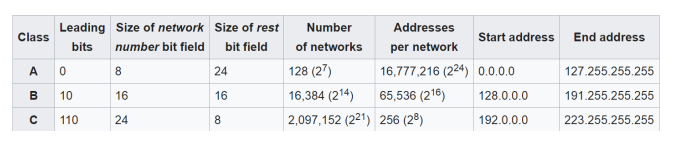
\includegraphics[width=\textwidth
]{images/ip-address-classes.png}
	\caption[Clases de direcciones IP]{Clases de direcciones IP}
	\label{fig:ip-address-classes}
\end{figure}

Por convención, las direcciones IP se escriben como cuatro enteros decimales separados por puntos. Cada entero representa el valor decimal contenido en 1 byte de la dirección, comenzando por el bit más significativo.

\subsubsection{Forwarding de datagramas en IP}
Un datagrama se envía desde un host de origen a un host de destino, posiblemente pasando por varios routers en el camino. Cualquier nodo, ya sea un host o un enrutador, primero intenta establecer si está conectado a la misma red física que el destino. Para hacer esto, compara la parte de red de la dirección de destino con la parte de red de la dirección de cada una de sus interfaces de red.

Si hay alguna una coincidencia significa que el destino se encuentra en la misma red física que la interfaz y el paquete se puede entregar directamente a través de esa red.

Si el nodo no está conectado a la misma red física que el nodo de destino, entonces debe enviar el datagrama a un router. En general, cada nodo tendrá varias opciones de routers, por lo que debe elegir el mejor, o al menos uno que tenga una posibilidad razonable de acercar el datagrama a su destino. El router que elige se conoce como \textbf{next hop}. El router encuentra el siguiente salto correcto consultando su tabla de reenvío. La tabla de forwarding es conceptualmente solo una lista de pares \(<NetworkNum, NextHop>\).

Normalmente, también hay un enrutador predeterminado que se usa si ninguna de las entradas en la tabla coincide con el número de red de destino.

El direccionamiento jerárquico ha mejorado la escalabilidad de una gran red dividiendo la dirección en partes de red y host. Los enrutadores ahora contienen tablas de reenvío que enumeran solo un conjunto de números de red en lugar de todos los nodos de la red.

\subsection{Subnetting}
\textbf{Subnetting} proporciona un primer paso para reducir el número total de números de red que se asignan a una tabla de forwarding. La idea es tomar un solo número de red IP y asignar las direcciones IP con ese número de red a varias redes físicas, que ahora se denominan subredes. Varias cosas deben hacerse para que esto funcione. Primero, las subredes deben estar cerca unas de otras. Esto se debe a que en un punto distante de Internet, todas parecerán una sola red, teniendo solo un número de red entre ellas. Esto significa que un enrutador solo podrá seleccionar una ruta para llegar a cualquiera de las subredes, por lo que es mejor que todas estén en la misma dirección general.

Se agrega a la identificación de un host una \textbf{máscara de subred} que permitirá identificar la red a la que pertenece un host. De esta manera, podrá haber varios host con el mismo número de red pero pertenecen a distintas redes físicas. 

Cuando el host quiere enviar un paquete a una cierta dirección IP, lo primero que hace es realizar un AND bit a bit entre su propia máscara de subred y la dirección IP de destino. Si el resultado es igual al número de subred del host de envío, entonces sabe que el host de destino está en la misma subred y el paquete se puede entregar directamente sobre la subred.

Si los resultados no son iguales, el paquete debe enviarse a un enrutador para que se reenvíe a otra subred.

La tabla de forwarding de un enrutador también cambia ligeramente cuando introducimos el subnetting. Recordemos que anteriormente teníamos una tabla de forwarding que consistía en entradas de la forma \(<NetworkNum, NextHop>\). Para soportar el subnetting, la tabla ahora debe tener entradas de la forma \(<SubnetNumber, SubnetMask, NextHop>\). Para encontrar la entrada correcta en la tabla, el enrutador realiza un AND bit a bit entre la dirección de destino del paquete y la SubnetMask para cada entrada; si el resultado coincide con el SubnetNumber de la entrada, entonces esta es la entrada correcta para usar, y reenvía el paquete al enrutador indicado.

% Traducir el siguiente texto:
The forwarding table of a router also changes slightly when we intro-
duce subnetting. Recall that we previously had a forwarding table that
consisted of entries of the form hNetworkNum, NextHopi. To support sub-
netting, the table must now hold entries of the form hSubnetNumber,
SubnetMask, NextHopi. To find the right entry in the table, the router
ANDs the packet’s destination address with the SubnetMask for each
entry in turn; if the result matches the SubnetNumber of the entry, then
this is the right entry to use, and it forwards the packet to the next hop
router indicated.
% A español:
La tabla de forwarding de un enrutador también cambia ligeramente cuando introducimos el subnetting. Recordemos que anteriormente teníamos una tabla de forwarding que consistía en entradas de la forma \(<NetworkNum, NextHop>\). Para soportar el subnetting, la tabla ahora debe tener entradas de la forma \(<SubnetNumber, SubnetMask, NextHop>\). Para encontrar la entrada correcta en la tabla, el enrutador realiza un AND bit a bit entre la dirección de destino del paquete y la SubnetMask para cada entrada; si el resultado coincide con el SubnetNumber de la entrada, entonces esta es la entrada correcta para usar, y reenvía el paquete al siguiente enrutador indicado.

\subsubsection{Direcciones sin clases}
El subnetting tiene un contraparte, a veces llamado supernetting, pero más a menudo llamado \textbf{Classless Interdomain Routing} o \textbf{CIDR}, pronunciado "cider". CIDR lleva la idea de subnetting a su conclusión lógica al eliminar las clases de direcciones por completo. 

El subnetting solo nos permite dividir una dirección de clase entre múltiples subredes, mientras que CIDR nos permite fusionar varias direcciones de clase en una sola "supernet" y lo hace de una manera que evita que el sistema de enrutamiento se sobrecargue.


CIDR trata de equilibrar el deseo de minimizar el número de rutas que un enrutador necesita conocer contra la necesidad de asignar direcciones de manera eficiente. Para hacer esto, CIDR nos ayuda a agregar rutas. Es decir, nos permite usar una sola entrada en una tabla de forwarding para decirnos cómo llegar a muchas redes diferentes. Como se señaló anteriormente, lo hace rompiendo los límites rígidos entre las clases de direcciones.

CIDR requiere un nuevo tipo de notación para representar los números de red, o prefijos como se los conoce, porque los prefijos pueden tener cualquier longitud. La convención es colocar un /X después del prefijo, donde X es la longitud del prefijo en bits.

La capacidad de agregar rutas en los extremos de direcciones de la red como acabamos de ver es solo el primer paso

Si asignamos prefijos a los clientes de tal manera que muchas redes de clientes diferentes conectadas a la red del proveedor compartan un prefijo de dirección común y más corto, entonces podemos obtener una mayor agregación de rutas.

\subsubsection*{IP Forwarding y CIDR}
CIDR significa que los prefijos pueden tener cualquier longitud, desde 2 hasta 32 bits. Además, a veces es posible tener prefijos en la tabla de forwarding que "se superponen", en el sentido de que algunas direcciones pueden coincidir con más de un prefijo.

La regla en este caso se basa en el principio de "coincidencia más larga"; es decir, el paquete coincide con el prefijo más largo.

El algoritmo para encontrar eficientemente la coincidencia más larga entre una dirección IP y los prefijos de longitud variable en una tabla de forwarding utiliza un enfoque conocido como árbol PATRICIA.

\subsection{Addressing Translation (ARP)}
Uno de los principales problemas que falta resolver es que los datagramas IP contienen direcciones IP, pero el hardware de interfaz física en el host o enrutador al que desea enviar el datagrama solo comprende el esquema de direccionamiento de esa red en particular. Por lo tanto, necesitamos traducir la dirección IP a una dirección de nivel de enlace que tenga sentido en esta red (por ejemplo, una dirección Ethernet de 48 bits). Luego podemos encapsular el datagrama IP dentro de un frame que contenga esa dirección de nivel de enlace y enviarlo al destino final o a un enrutador que prometa reenviar el datagrama hacia el destino final.

Esto se puede lograr utilizando el Protocolo de Resolución de Direcciones (ARP). El objetivo de ARP es permitir que cada host en una red construya una tabla de asignaciones entre direcciones IP y direcciones de nivel de enlace. Dado que estas asignaciones pueden cambiar con el tiempo, las entradas se eliminan periódicamente. Esto sucede en el orden de cada 15 minutos. El conjunto de asignaciones almacenadas actualmente en un host se conoce como caché ARP o tabla ARP.


ARP aprovecha el hecho de que muchas tecnologías de red de nivel de enlace, como Ethernet, admiten broadcasting. Si un host desea enviar un datagrama IP a otro host (o a un enrutador) que sabe que está en la misma red, primero verifica si hay un mapeo en la caché. Si no se encuentra ningún mapeo, debe invocar el Protocolo de resolución de direcciones en la red. Lo hace transmitiendo una consulta ARP en la red. Esta consulta contiene la dirección IP de destino. Cada host recibe la consulta y verifica si coincide con su dirección IP. Si coincide, el host envía un mensaje de respuesta que contiene su dirección de nivel de enlace de regreso al originador de la consulta. El originador agrega la información contenida en esta respuesta a su tabla ARP.

La consulta también incluye la dirección IP y la dirección de nivel de enlace del host que envía. De esta manera, el host de destino puede aprender las direcciones de nivel de enlace y de IP del remitente y colocar esa información en su tabla ARP si es que ya no la tienen guardada.  Si el host ya tiene una entrada para ese host en su tabla, "actualiza" esta entrada para que dure más tiempo.

El formato del paquete ARP para mapeos de direcciones IP a Ethernet contiene:
\begin{itemize}
    \item Un campo \textbf{HardwareType}, que especifica el tipo de red física.
    \item Un campo \textbf{ProtocolType}, que especifica el protocolo de capa superior
    \item Campos \textbf{HLen} ("longitud de dirección de hardware") y \textbf{PLen} ("longitud de protocolo"), que especifican la longitud de la dirección de capa de enlace y la dirección de protocolo de capa superior, respectivamente
    \item Un campo \textbf{Operation}, que especifica si se trata de una solicitud o una respuesta
    \item Las direcciones de hardware (Ethernet) y protocolo (IP) de origen y destino
\end{itemize}

\subsection{Host Configuration (DHPC)}
Las direcciones IP, no solo deben ser únicas en una interred determinada, sino que también deben reflejar la estructura de la misma. Como se señaló anteriormente, contienen una parte de red y una parte de host, y la parte de red debe ser la misma para todos los hosts en la misma red. Por lo tanto, no es posible configurar la dirección IP una vez en un host cuando se fabrica, ya que eso implicaría que el fabricante sabía qué hosts iban a terminar en qué redes, y significaría que un host, una vez conectado a una red, nunca podría moverse a otra. Por esta razón, las direcciones IP deben ser reconfigurables.

El método principal de configuración utiliza un protocolo conocido como \textbf{Protocolo de configuración dinámica de host (DHCP)}. DHCP se basa en la existencia de un servidor DHCP que es responsable de proporcionar información de configuración a los hosts. Existe al menos un servidor DHCP por dominio administrativo.

El servidor DHCP mantiene un grupo de direcciones disponibles que entrega a los hosts a pedido. Esto reduce considerablemente la cantidad de configuración que debe realizar un administrador, ya que ahora solo es necesario asignar un rango de direcciones IP (todas con el mismo número de red) a cada red.

Para contactar a un servidor DHCP, un host recién iniciado o conectado envía un mensaje \textbf{DHCPDISCOVER} a una dirección IP especial (255.255.255.255) que es una dirección de broadcast en IP. Esto significa que será recibido por todos los hosts y enrutadores en esa red. (Los enrutadores no reenvían dichos paquetes a otras redes, evitando la difusión a toda Internet). En el caso más simple, uno de estos nodos es el servidor DHCP para la red. El servidor respondería entonces al host que generó el mensaje de descubrimiento.

Sin embargo, no es realmente deseable requerir un servidor DHCP en cada red, porque esto implica una gran cantidad de servidores que deben configurarse correctamente y de manera consistente. Por lo tanto, DHCP utiliza el concepto de un agente de retransmisión. Hay al menos un agente de retransmisión en cada red, y se configura con solo una pieza de información: la dirección IP del servidor DHCP. Cuando un agente de retransmisión recibe un mensaje DHCPDISCOVER, lo envía en unicast al servidor DHCP y espera la respuesta, que luego enviará al cliente solicitante.

El mensaje se envía realmente utilizando un protocolo llamado \textbf{Protocolo de Datagrama de Usuario (UDP)} que se ejecuta sobre IP.

En el caso en que DHCP asigne dinámicamente direcciones IP a los hosts, no pueden mantener las direcciones indefinidamente, ya que esto eventualmente causaría que el servidor agote su pool de direcciones. Al mismo tiempo, no se puede depender de que un host devuelva su dirección, ya que podría haberse bloqueado, desconectado de la red o apagado. Por lo tanto, DHCP permite que las direcciones se asignen por un período de tiempo determinado. Una vez que la asignación expire, el servidor es libre de devolver esa dirección a su pool. Un host con una dirección asignada necesita renovar el arriendo periódicamente si todavía está conectado a la red y funciona correctamente.

\subsection{Error Reporting (ICMP)}
IP siempre se configura con un protocolo complementario, conocido como \textbf{Protocolo de mensajes de control de Internet (ICMP)}, que define una colección de mensajes de error que se envían al host de origen cada vez que un enrutador o host no puede procesar un datagrama IP correctamente.

ICMP también define mensajes de control que un enrutador puede enviar de vuelta a un host de origen. Uno de los mensajes de control más útiles, llamado ICMP-Redirect, le dice al host de origen que hay una mejor ruta hacia el destino.

\subsection{Virtual Networks and Tunneling}

Las empresas con varios sitios tienden a construir redes privadas alquilando lineas de compañias electrónicas para interconectarlos. En estas redes, la comunicación se restringe a los sitios de la corporación, lo cual es deseable por razones de seguridad. Para hacer una red privada virtual, las lineas de transmisión alquiladas - que no son compartidas con otras corporaciones - serían reemplazadas por algún tipo de red compartida. Un circuito virtual (VC) es un reemplazo razonable para una linea alquilada porque aún provee una conexión lógica punto a punto entre los sitios de la corporación.

También es posible proporcionar una función similar utilizando una red IP, una interred, para proporcionar la conectividad. Sin embargo, no podemos simplemente conectar los sitios de las diversas corporaciones a una sola interred porque eso proporcionaría conectividad entre la corporación X y la corporación Y, lo que deseamos evitar. Para resolver este problema, necesitamos introducir un nuevo concepto, el \textbf{túnel IP}.

Podemos pensar en un túnel IP como un enlace virtual punto a punto entre un par de nodos que están separados por un número arbitrario de redes. El enlace virtual se crea dentro de un enrutador \(R_1\) en la entrada del túnel al proporcionarle la dirección IP del enrutador \(R_2\) en el otro extremo del túnel. Cada vez que \(R_1\) desea enviar un paquete por este enlace virtual, encapsula el paquete dentro de un datagrama IP. La dirección de destino en el encabezado IP es la dirección de \(R_2\), mientras que la dirección de origen es la de \(R_1\).

Una vez que el paquete sale de \(R_1\), parece al resto del mundo como un paquete IP normal destinado a \(R_2\), y se reenvía en consecuencia. Todos los enrutadores en la interred lo reenvían utilizando medios normales, hasta que llega a \(R_2\). Cuando \(R_2\) recibe el paquete, encuentra que lleva su propia dirección, por lo que elimina el encabezado IP y mira la carga útil del paquete. Lo que encuentra es un paquete IP interno cuya dirección de destino está en una red interna. \(R_2\) ahora procesa este paquete como cualquier otro paquete IP que recibe. Dado que \(R_2\) está directamente conectado a esta red, reenvía el paquete a esa red.

Este mecanismo tiene sus desventajas. Una es que aumenta la longitud de los paquetes; esto podría representar una pérdida significativa de ancho de banda para paquetes cortos. Los paquetes más largos pueden estar sujetos a fragmentación, que tiene su propio conjunto de inconvenientes. También puede haber implicaciones de rendimiento para los enrutadores en cada extremo del túnel, ya que necesitan hacer más trabajo que el reenvío normal al agregar y eliminar el encabezado del túnel.

Finalmente, existe un costo de administración para la entidad administrativa que es responsable de configurar los túneles y asegurarse de que sean manejados correctamente por los protocolos de enrutamiento.